\graphicspath{{images/}{images/logos/}}

\begin{frame}{Meine Tätigkeiten}
	\begin{itemize}
		\item Scrum Master
			\subitem Koordination
			\subitem Ansprechpartner
			\subitem ....
		\item Einarbeiten in den Simulator
			\begin{itemize}
				\item Verstehen wie Simulationen ablaufen
				\item Was muss angepasst werden für neue Agenten
			\end{itemize}
		\item Erweitern des Simulators um Horse
	\end{itemize}
\end{frame}  

\begin{frame}{Ablauf der Simulation}
	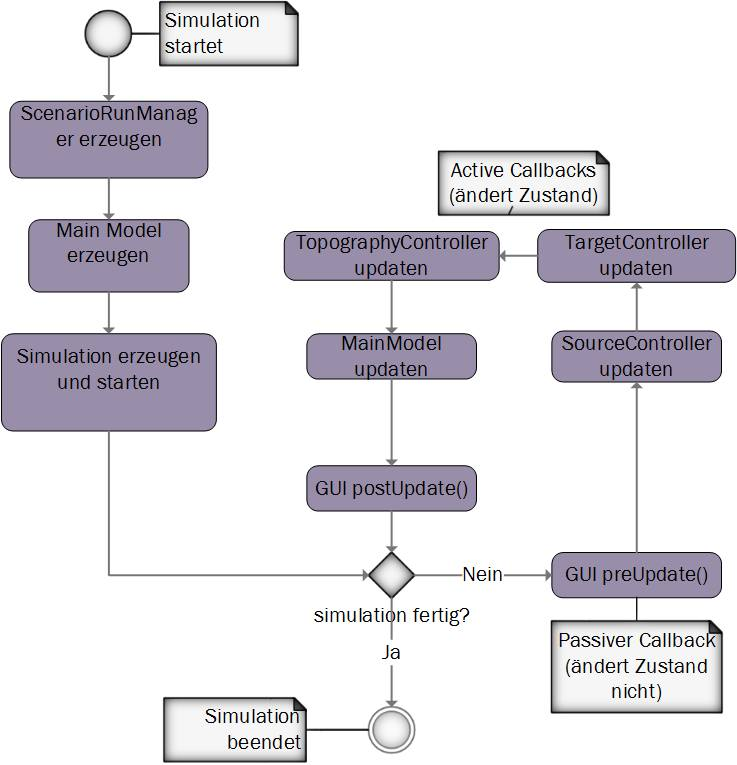
\includegraphics[width=250,height=240]{./simul.png}
\end{frame}

\begin{frame}{Fazit}
	\begin{itemize}
		\item 	\underline{Fand ich gut:} \newline $\underline{}$
			\begin{itemize}
				\item Gelegenheit an einem größeren Projekt zu arbeiten
				\item Gute Zusammenarbeit (skype und trello)
			\end{itemize}
		\newline
		\item \underline{Kann besser sein:} \newline $\underline{}$
			\begin{itemize}
				\item Einbezug in aktuelle Änderungen des Codes
				\item Regelmäßiger Treffen \newline
			\end{itemize}
		\item \underline{Anteil Schätzung:} $\underline{}$ \tab 19\%
	\end{itemize}
\end{frame}